\beginsong{Zogen einst fünf wilde Schwäne}[wuw={1917, Text aus dem Litauischen, übersetzt von Karl Plenzat, Musik aus Masuren}, pfii={63}, bo={444}]

\markboth{\songtitle}{\songtitle}

\beginverse
\endverse

\centering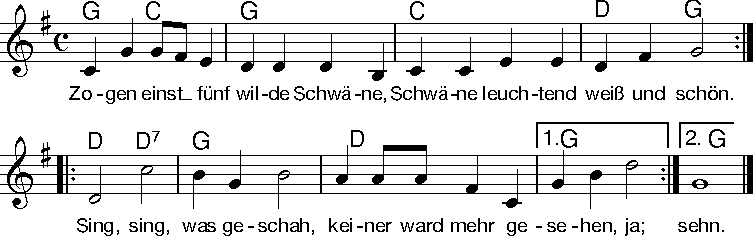
\includegraphics[width=1\textwidth]{Noten/Lied104.pdf}	

\beginverse
\lrep \[G]Wuchsen \[C]einst fünf \[G]junge Birken, \[C]grün und frisch am \[D]Baches\[G]rand. \rrep 
\lrep \[D]Sing, \[D7]sing, \[G]was geschah, \[D]keine in Blüte \[G]stand. \rrep 
\endverse

\beginverse
\lrep ^Zogen ^einst fünf ^junge Burschen ^stolz und kühn zum ^Kampf hi^naus. \rrep 
\lrep ^Sing, ^sing, ^was geschah, ^keiner kam mehr nach ^Haus. \rrep 
\endverse

\beginverse
\lrep ^Wuchsen ^einst fünf ^junge Mädchen, ^schlank und schön am ^Memel^strand. \rrep 
\lrep ^Sing, ^sing, ^was geschah, ^keine den Brautkranz ^wandt. \rrep 
\endverse

\endsong

\beginscripture{}
Das Lied handelt von den existentiellen Folgen des Krieges und wurde in den 1920er Jahren durch die Jugendbewegung in ganz Deutschland bekannt gemacht. Der Inhalt deutet die einschneidenden Folgen des Krieges an: Die Schwäne stehen für die Männer, die weg 'fliegen', nicht mehr zurück kommen und ihr Frauen ehelos zurück lassen. 
\endscripture

\begin{intersong} 

\end{intersong}